%\chapter{Apports de SDN aux data centres}
%Ce chapitre démontre les apports de SDN au sein des data centres par rapports aux problématiques présentées précédemment.

\section{Scénarios d'utilisation}

Un système cloud qui s'intègre de façon transparente et dynamique avec un réseau programmable (grâce à SDN) peut fournir une importante plus-value à ses opérateurs et à leurs abonnés (consommateurs finaux et entreprises). Aujourd'hui la connectivité seule ne suffit pas, les utilisateurs réclament une variété de services hébergés dans le cloud, et cela exige des réseaux la capacité de fournir la connectivité correcte à l'application souhaitée. C'est dans ce cadre que  la réelle valeur d'un cloud à réseau dynamiquement programmable  devient visible.
%A cloud system that integrates seamlessly with a real-time, programmable network – enabled by Service Provider SDN – can provide significant value to network operators and their subscribers (both consumers and enterprises). Today, most subscribers do not rely on connectivity alone. Instead, they demand a wide range of services that are cloud-hosted, and they require the network to play a role in offering the right connectivity for the desired application. This is where the real value of a Service Provider SDN-based, real-time programmable network and cloud becomes apparent.

Cette capacité permet de découper le réseau en tranches et offrir aux clients leurs morceaux dédiées et personnalisés. Il existe une variété de scénarios imaginables  à partir de ce concept de diviser le réseau pour convenir à différents applications et besoins.
%A “meta” use case is the ability to slice and offer consumers/enterprises a piece of the network-plus-cloud for their dedicated, personalized use. There are multiple variants of use cases that are based on this concept of the ability to slice networks to suit different applications and enterprise needs.

Un des cas d'utilisation est l'infrastructure virtuelle d'entreprise, dans laquelle un portail basé sur SDN peut être étendu selon les particularités de l'organisation. La solution associe la coordination riche d'un contrôleur cloud et d'un contrôleur SDN. Cela permet l'instanciation, la réplication et la migration du réseau et services basés cloud dans la meilleure localisation disponible, en fonction des requis tenants, de la congestion globale du réseau et de la disponibilité de ressources. Cette solution conforme à l'idéal de ne pas limiter le cloud avec les contraintes physiques du data centre, implémentant un suivi de flux et un renforcement de politiques dans un niveau logique pour le cloud. Cela peut englober plusieurs data centres, quelle que soit leur localisation géographique dans l'infrastructure du réseau.
%One such case is the Virtual Enterprise IT Infrastructure – in which an SDN-based gateway can be extended to the enterprise premises. The solution features tight coordination between a feature-rich cloud controller and an SDN controller. This enables the instantiating, replicating and migrating of network and cloud-based services to the best available location, based on the tenant’s requirements, overall network congestion and cloud availability. True to the ideal of not tying cloud services to the constraints of a physical data center, this solution implements flow tracking and policy enforcement at a “logical” cloud level. This encompasses multiple operator data centers, irrespective of their geographic locations and the network infrastructure connecting them.


%Another case is the virtual home gateway. This is an example of virtualizing some of the functions of a traditional home gateway and hosting them in a Network-enabled Cloud. Virtualization reduces the complexity of the home gateway by moving most of the sophisticated functions into the network. As a result, operators can prolong the home gateway refreshment cycle, cut maintenance costs and reduce time to market for new services. The most important aspect of this solution, however, is that it gives the network visibility to all the devices that were traditionally hidden behind the home gateway. This opens up significant revenue opportunities through the ability to offer services that are personalized in a much more granular way.



Un des scénarios les plus traditionnels de l'intégration des services dynamiques avec SDN consiste à en resserrer l'interaction entre le réseau et le cloud. Pour les services "inline" tels que filtrage, modification des entêtes et \gls{nat}, les opérateurs utilisent diverses "appliances", ou d'autres services pour gérer le trafic utilisateur. Ces services sont hébergés dans du matériel physique ou en machines virtuelles. L’enchaînement de services est nécessaire pour router le trafic client à travers ces services. Les solutions traditionnelles sont soit statiques ou très limitées en flexibilité et \gls{scalability}.
%The more traditional and now widely accepted Service Provider SDN use case of dynamic service chaining* itself relies on tight interaction between the network and the cloud. For inline services, such as content filtering, header enrichment, firewalls and Network Address Translation (NAT), operators use different appliances, or value-added services to manage subscriber traffic. These inline services can be hosted on dedicated physical hardware or on virtual machines (software appliances running in a virtualized cloud environment). Service chaining is required to route certain subscriber traffic through more than one such service. Solutions currently available are either static or their flexibility is significantly limited by scalability inefficiencies.

%Dynamic service chaining can optimize the use of extensive high-touch services by either selectively steering traffic through specific services or bypassing them completely. This can provide capex savings through efficient use of capacity. Greater control over traffic and the use of subscriber-based selection of inline services can lead to the creation of new offerings and new ways to monetize networks.

%The Network-enabled Cloud provides the necessary virtual resources for software appliances, whether on dedicated physical hardware or on virtual machines, and supports efficient distribution of these resources wherever needed in the network, such as to best meet latency requirements. 

%Dans un Cloud habilité réseau, l'extension des applications peut être achevée avec la demande de ressources virtuelles. Scaling a software appliance can be achieved either by requesting more cloud capacity in the Network-enabled Cloud or by requesting virtual resources in a centralized cloud data center. The flexibility of the distributed cloud is greatly enhanced using the Service Provider SDN real-time control mechanism, in which software appliances can be moved within or between clouds while preserving the networking attributes and requirements.

Dans le chapitre précédent, les principaux défis des réseaux traditionnels pour fonctionner en mode Cloud ont été détaillés. Un résumé simplifié des principales difficultés a été proposé. Les prochaines sections, traitent ces points et illustrent comment ces objectifs peuvent être atteints en utilisant SDN.


\section{Complexité vs Agilité}

La complexité et l'agilité sont des éléments qui sont fortement accoupler doivent donc être étudiés ensemble. En effet, la complexité est une pour atteindre les objectifs d'agilité, qui en revanche provoque un niveau plus haut de complexité dans l'approche réseau traditionnelle. Cet impasse a pu être observé dans les scénarios présentés précédemment. 

Les architectures réseaux implémentant SDN proposent d'aplatir physiquement la topologie avec l'interconnexion de tous les élément à un \gls{fabric} pour à la fois simplifier le réseau et gagner en agilité. L'image ci-dessous visualise cette proposition. Le contrôleur SDN peut être programmé pour reproduire logiquement l'infrastructure souhaitée par tenant. 

\begin{figure}[h]
\begin{center}
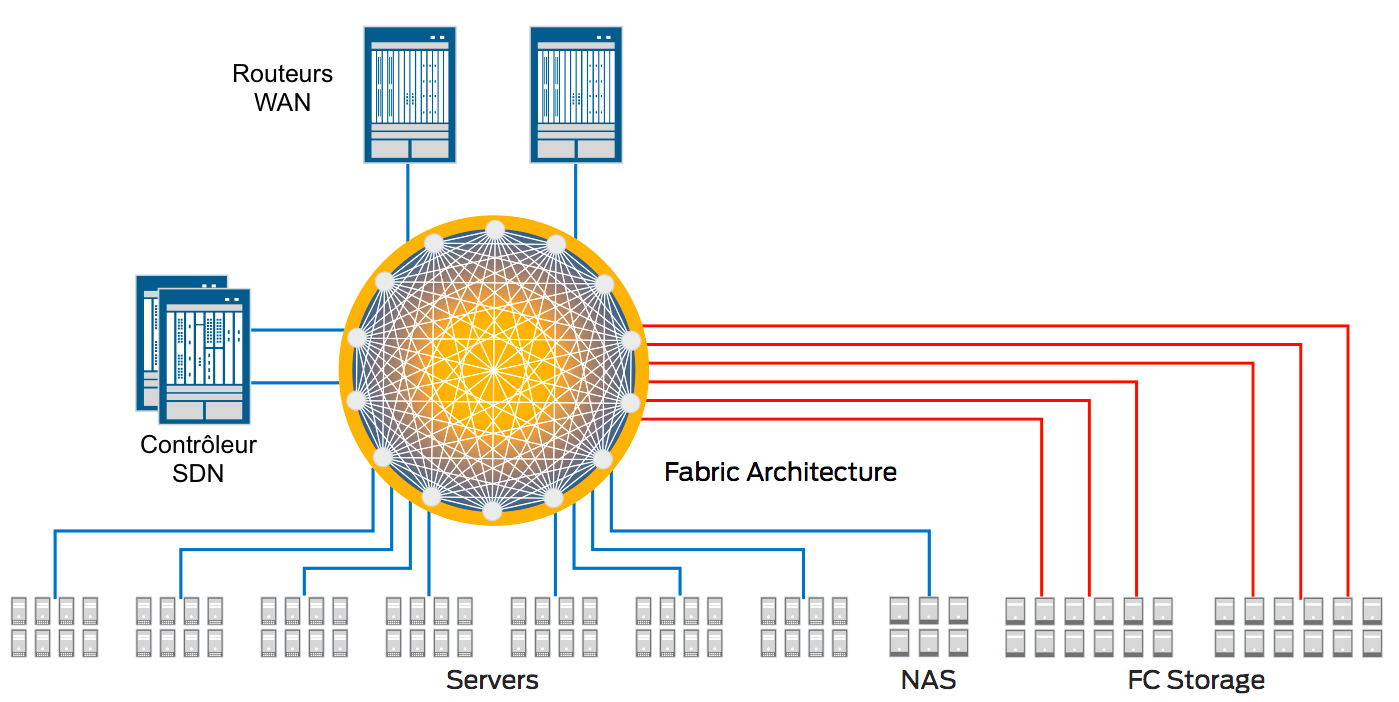
\includegraphics[width=0.8\textwidth]{images/RefArchiSDN} 
\caption{Topologie réseau simplifiée. \cite{cloudReadyNetworkJuniper}} \label{RefArchiSDN}
\end{center}
\end{figure} 

Avec les solutions SDN, les changements sur le réseau sont traité par un processus complètement automatisé qui peut réagir instantanément. Ainsi que comme on fait pour les VMs, SDN permet de créer des templates pour les réseaux logiques des tenants qui peuvent être facilement instanciés implémentant tous les aspects réseaux automatiquement. 
%With the Nuage Networks solution, changes are handled by a fully automated process that can react instantaneously. This makes network operations much simpler across an open cloud environment.

Les templates peuvent être réutilisés plusieurs fois, si l'opération doit être répétée. Les solutions SDN peuvent créer le réseau nécessaire et fournir l'isolation complète entre tenants, ce qui simplifie considérablement les opérations réseaux au sein des data centres. 
%The Nuage Networks VSP automates the full instantiation of the tenant networking requirements through SDN programmability and abstraction.
%The template can be used as many times as required, should this operation need to be repeated multiple times. The Nuage Networks VSP solution instantiates the necessary networking and provides full isolation between tenants and through the robust implementation of SDN technology pillars, which simplifies the operation of the data center network substantially.

Cela apporte une réponse plus rapide aux demandes des clients. La simplification opérationnelles grâce à la capacité de programmation et abstraction SDN élimine les opérations manuelles très susceptibles aux erreurs, avec une meileure efficacité du réseau et plus de profit.
%Faster response time to customer demands, which results in much higher customer satisfaction
%• Simplified business operations through templates that are created once and used many times
%• Operational simplification through automation, with SDN programmability and abstraction
%• Elimination of tedious manual operations, which in turn eliminates the potential for human errors associated with implementation and modification of customer tenant configurations
%• Higher data center network and server efficiency through elimination of bottlenecks, ultimately resulting in lower CAPEX and higher profitability

\section{Sécurité}

La sécurité dans un data centre Cloud doit protéger le trafic entre les clients et serveurs, le trafic entre les machines virtuelles dans les servuers ainsi que le trafic entre serveurs (physiques ou virtuels) et applications ou systèmes dans d'autres data centres. La capacité d'extension est requis de sécurité essentiel dans ces environnements. 



%Security administrators in a cloud-ready data center must protect client-to-server traffic, traffic between virtual machines on servers, and traffic between physical and virtual servers, applications, and systems in other data centers . The ability to scale is a primary security requirement in these environments. 

L'importante croissance de l'accès utilisateur ainsi que de la sophistication des menaces de sécurité dans un data centre Cloud exigent une visibilité étendue du réseau et la mise en place des protections associées. Les solutions de sécurité doivent à la fois renforcer les politiques de manière consistante et rester flexibles pour assurer l'adaptation du réseau aux divers usages.

%Increasing user access and the rising sophistication of security threats in a cloud-ready data center also require expanded visibility into threat vectors and related protection . at the same time, security solutions still need to consistently enforce policies, while remaining flexible to adapt to the changes in traffic volumes and data flows that occur because of virtualization, web 2 .0 applications, and cloud services . appropriate policies affect the availability of business critical applications and operations .

Pour aborder ces défis, la sécurité d'un cloud doit réunir des capacités telles que \gls{scalability}, monitoring et contrôles renforcés. Les services de sécurité doivent être consolidés et coordonnés pour complimenter la simplification  et la mutualisation agile du réseau. Cette approche améliore la flexibilité et efficacité du système entier.
%To address these challenges, capabilities such as scale, visibility, and enforcement controls must work together to comprehensively secure a cloud-ready data center . Security services must be consolidated and pooled in a coordinated fashion to complement the simplification and sharing of the network . This approach enhances the flexibility and efficiency of the entire solution .

SDN propose des moyens pour fournir de services dynamiques de sécurité et répondre aux requis de performances tout en accommodant les évolutions futures à la demande. De services tels que supervision, filtrage, détection et prévention d'intrusion et VPNs sont consolidés dans une plateforme extensible avec de ressources affectées dynamiquement. La solution améliore également chaque service de sécurité en augmentant dynamiquement leur capacité d'accès à tout flux de trafic au sein du \gls{fabric} réseau.
%Big Tap enhances the functionality of each network security and monitoring appliance by dynamically extending its reach to any traffic flow within the network fabric. 
%Juniper networks has developed high- performance, cloud-enabled dynamic security services to meet today’s security and performance requirements, while accommodating future on-demand growth . Services such as application identification and monitoring, stateful firewall, intrusion detection and prevention, and VPns are consolidated on an expandable platform that flexibly and dynamically assigns resources as needed . 

Les services de sécurité doivent être conscient des applications, tout en étant mobiles. L'interface de programmation fournie avec SDN permet l'interaction avec les hyperviseurs assurer la sécurité inter-VMs. Les applications peuvent déployer un ensemble de politiques de sécurité à partir des hyperviseurs et à travers le \gls{fabric} réseau avec l'établissement d'un lien entre les couches virtuelles et physiques. 
%Security services must be application- and identity-aware, while providing the mobile workforce with secure access to data center applications . Juniper solutions now include integrated and comprehensive vGw Series virtual machine security capabilities for securing virtualized data centers . Businesses can deploy a consistent set of security policies and services from the hypervisor all the way across the network fabric, bridging virtual and physical network layers . 

Comme résultat, les consommateurs peuvent apercevoir la complète de la virtualisation, tout en étant protéger contre les risques de sécurité associés. SDN franchi les deux principaux préoccupations concernant les plateformes Cloud : la sécurité et le contrôle. Le réseau, ayant contact à tous les éléments de l'infrastructure, est le meilleur endroit pour placer la sécurité et la gestion. Avec SDN, ces défis peuvent être abordés pour libérer le Cloud Computing. 
%As a result, customers can realize the full value of virtualization, while protecting against the associated security risks .

%The network is the best place to secure and manage the cloud: The two biggest barriers to broader use of cloud computing remains security and control (see Exhibit 2). Many IT managers are unclear as to how to secure and manage resources that they no longer own, and are not on-premises. Pushing control and security points to the network allows IT managers to meet these challenges. The network is the only IT asset that touches every other IT resource.
